\documentclass[10pt,conference,compsocconf]{IEEEtran}

%\usepackage{times}
%\usepackage{balance}
\usepackage{url}
\usepackage{graphicx}
\usepackage{amsmath}
\usepackage{svg}
\usepackage{hyperref}
\usepackage{float}

\begin{document}
\title{MINION vs BERT: Efficient Fine-Tuning}

\author{
  Gero Embser, Carlos Vonessen, Leo Widmer\\
  Banana-Fueled NN\\
  Department of Computer Science, ETH Zurich, Switzerland
}

\maketitle

\begin{abstract}
The past decades have seen an explosion in the use of microblogging and text messaging as popular communication channels. This rapid growth has resulted in an unprecedented volume of data, creating a pressing need for automated methods to analyze and understand the sentiments expressed in text. However, state-of-the-art methods are often expensive to train and exhibit overconfidence when faced with unseen dataset distributions. Parameter-efficient transfer learning (PETL) attempts to reduce the training cost associated with training large models, but often still requires significant computational resources to train models. In this paper, building on previous work, we implement a novel MINIature Orthogonal Network (MINION), that trains a small sequence-to-sequence recurrent neural network (RNN) alongside a large frozen transformer model, thus avoiding backpropagation through the larger transformer. We show that MINION requires lower training costs compared to previous implementations and full fine-tuning while reducing model overconfidence and maintaining high accuracy for text sentiment classification.

\end{abstract}

\section{Introduction}

Text sentiment analysis is a problem that has been widely approached with neural networks (NN) and in recent years specifically large language models (LLM) \cite{roberta, nguyen2020bertweet, gpt3, devlin2018bert}. LLMs such as RoBERTa \cite{roberta} create high-accuracy predictions for a wide range of NLP tasks and have become the standard in recent years. However, LLMs require very large amounts of data, high computational resources, and are very sensitive to choices in hyperparameters. Lacking time and resources, these difficulties make training an LLM or only fine-tuning it untenable in most cases. Research into parameter-efficient transfer learning (PETL) aims to address these issues. Instead of fine-tuning a full model, PETL methods introduce a few additional parameters to a pre-trained model or train a small subset of model weights, to adapt a pre-trained model to a specific task. Recently, the implementation of a REcurrent ADaptation (READ) model, that uses an RNN as a side model to a frozen LLM, has shown a significant reduction in training cost while exceeding the accuracy of fully finetuned models on several NLP tasks \cite{read}. A further complication of modern neural networks is that they often exhibit overconfidence in their predictions \cite{guo2017calibration}, i.e. generate high probabilities for predictions with lower accuracy rate. Models with bad calibration reduce the interpretability of their outputs and increase risk in safety-critical applications \cite{vaicenavicius2019evaluating, guo2017calibration}. \\
Faced with the task of training a well-calibrated, high-accuracy model with limited time and resources that is able to compete with an industry-standard like RoBERTa, we build on the side-tuning approach first implemented in READ \cite{read}.
\begin{enumerate}
    \item We expand on READ by implementing a new side model configuration, that freezes the transformer and trains only a sequence-to-sequence RNN,
    \item We show higher accuracy using the same RNN hidden layer size and fewer parameters in our side model compared to READ,
    \item We show that our approach yields a significant reduction in training costs compared to full fine-tuning while maintaining high accuracy and reducing calibration error.
\end{enumerate}


\section{Models and Methods}
\label{sec:models-methods}

An overview of the implemented models can be found in Table~\ref{tab:model-overview}.

\subsection{Baseline Models}
To evaluate the performance of our approach, we implement two conventional baseline models and one baseline model more specific to our implementation.

\subsubsection{FastText}
In the context of natural language processing (NLP) tasks, like sentiment analysis, FastText \cite{bojanowski2017fasttext} is a common and straightforward baseline. It is a shallow neural network as it only has two layers: An embedding layer and a classification layer. In contrast to most state-of-the-art models, it is not based on a transformer architecture but relies on the "bag-of-words" model. The text embeddings are averaged together to create a fixed-length representation of the input. It then uses a shallow NN for classification. Compared to LLMs, it has extremely low training costs and very high inference speeds. This makes it a good baseline, as using it is often an attractive alternative in NLP tasks when one has limited data and computational resources.

\subsubsection{BERTweet}
The ubiquitous use of LLMs in NLP tasks has made such models meaningful baselines. In this paper, we fully fine-tune the BERTweet model \cite{nguyen2020bertweet} on our dataset. BERTweet is already fine-tuned on Twitter data and is based on the BERT architecture \cite{devlin2018bert}. In using BERTweet as a baseline, we explore what model performance and computational costs are created by using an out-of-the-box LLM and fine-tuning it for our specific task. BERTweet is much more computationally expensive than FastText but also achieves significantly higher accuracies on most NLP tasks \cite{nguyen2020bertweet}. Furthermore, fully fine-tuned BERTweet is an attractive baseline to us, as we use BERTweet as a part of our own implementations which gives a direct comparison for accuracy, computational cost, and calibration.

\subsubsection{READ}
As our final base model we use the REcurrent ADaptation (READ) model presented in \cite{read}, on whose principles we build our own implementation. It is useful as a final base model, as it is closest to our own implementation and thus clearly shows the difference our additions make. The goal of READ is to fine-tune a large pre-trained transformer $\mathcal T$ efficiently in terms of memory and energy consumption. Here, we explain how READ works if $\mathcal T$ has only an encoder and no decoder. $\mathcal T$ is frozen all throughout training. First, a forward pass is executed on $\mathcal T$ where one caches the results of all the layers, i.e. states $\phi_1, \dots,\phi_N$. If we had fine-tuned the transformer directly we could obtain the desired states $\phi'_1,\dots,\phi'_N$. Instead of doing this, READ tries to approximate so-called corrections $\delta\phi_i:=\phi'_i-\phi_i$, which we then can add to $\phi_i$ to obtain the fine-tuned $\phi'_i$. These approximated corrections, denoted as $h_i$, are computed using an RNN, which is unrolled alongside $\mathcal T$. Starting with a sequence of length $m$, we iterate through the states for $i$ from 1 to $N$ and compute
\begin{align}
    h_i^\alpha = \mathcal N\left(\phi_i^\alpha, h_{i-1}^\alpha\right)\ \forall\alpha\in\{1,...,m\},
\end{align}
where $\mathcal N$ is one step in the time of the RNN. We assume the embedding state needs no correction, so $h_0=0$. In the end, we map $h_N$ to the dimension of the output state $\phi_N$ and return the approximation $\phi_N + h_N\approx\phi'_N$. The output sequence is then averaged and fed into a linear classifier. The basic structure is again illustrated in Figure~\ref{fig:readarchitecture}.
We implement the RNN as a bidirectional RNN using Gated Recurrent Units (GRUs). As a pre-trained network $\mathcal T$ we use BERTweet \cite{nguyen2020bertweet}.

\begin{figure}
  \centering
  \includesvg[width=0.5\columnwidth]{READ_diagram.svg}
  \caption{The READ architecture that we use for our experiments.}
  \label{fig:readarchitecture}
\end{figure}

\subsection{MINION}
Our model works similarly to READ but uses a different function $\mathcal N$ in the computation of the corrections $h_i$. Here, $\mathcal N$ first computes $x_i=\mathcal F\phi_i + h_{i-1}$, where $\mathcal F$ is a linear layer, and then feeds the sequence $x_i=x_i^1,...,x_i^m$ into a sequence-to-sequence RNN which returns $h_i^1,...,h_i^m=h_i$. In the current description of READ, $h_i^\alpha$ and $h_i^{\alpha'}$ for $\alpha\neq\alpha'$ are independent of each other. In contrast, by using a sequence-to-sequence RNN, we expect that MINION efficiently captures the dependency structure arising from natural text, thus requiring fewer parameters for similar performance. See Figure \ref{fig:informationflow} for the difference between READ and MINION in terms of information flow.  Fewer parameters will also prevent the very large transformer model from overfitting on the relatively small data set. We call our RNN configuration an orthogonal RNN, as it also transmits information orthogonally to the transformer layers, in contrast, we call the original READ network a parallel RNN.\\
The sequence-to-sequence RNN is implemented with bidirectional Gated Recurrent Units (GRUs). We experiment with hidden sizes much smaller than in the original READ paper \cite{read}, beginning at 8 and increasing through successive powers of two until 256, which was the hidden size selected in the original paper.
As the pre-trained network we use BERTweet \cite{nguyen2020bertweet}.

\begin{figure}[htbp]
  \centering
  \includesvg[width=0.75\columnwidth]{information_flow.svg}
  \caption{Information flow of READ vs. that of MINION.}
  \label{fig:informationflow}
\end{figure}

\subsection{Data}
The data used for training the models is provided to us by the Data Analytics Lab of ETH Zurich as a part of the Text Sentiment Classification Competition in the Computational Intelligence Lab 2023. The unprocessed data consists of 2.5 million tweets, where exactly half are labeled to have positive sentiment, and the other half are labeled with negative sentiment. The data is anonymized, meaning that references to specific users, for example, "\texttt{@realDonaldTrump}" have been replaced with the tag "\texttt{<user>}". Any URLs in a tweet have also been replaced with the tag "\texttt{<url>}".\\
We processed the data to remove duplicate tweets, which leaves 1,127,628 positive sentiment tweets and 1,142,785 negative sentiment tweets. Furthermore, since hashtags often contain a lot of the sentiment expressed in the text, we used an automated word separation library\footnote{\url{https://github.com/grantjenks/python-wordsegment}} based on \cite{segaran2009beautiful} to convert hashtags into normal text, i.e. "\texttt{<user> omg \#ilovethislab}" becomes "\texttt{<user> omg i love this lab}". This preprocessing step was done to increase the model's semantic understanding of the hashtags. FastText especially profits from this, as it uses a bag-of-words implementation and thus does not understand hashtags. The other models are predominantly trained on normal text and thus also stand to benefit from converting the hashtags to simple words.

\subsection{Energy Consumption}
To compare the cost of training each model we evaluate the approximate energy consumption and memory utilisation of each model during training.\\
We calculate estimated energy consumption based on the implementation presented in \cite{read}. We track GPU utilization $u_i$ (in percent) and memory usage $m_i$ (in MiB) every ten seconds during training. We further assume a linear relationship between power consumption and GPU utilization and use $p_0 = 0.4$kW \footnote{See this \href{https://www.nvidia.com/content/dam/en-zz/Solutions/Data-Center/a100/pdf/nvidia-a100-datasheet-us-nvidia-1758950-r4-web.pdf}{NVIDIA datasheet}} as the maximum power utilization constant. Using $H$ as the number of hours an experiment runs, we approximate the energy consumption $E$ (kWh) with the average $u_i$ value
\begin{align}
    E = \int_0^H  p_0 \frac{u(t)}{100}dt
    \approx \frac{H}{360H}\sum_i \frac{p_0 \cdot u_i}{100}
    &= \frac{p_0}{36000} \bar U
\end{align}
Here $\bar U=\sum_i u_i$ and one gets the 360, from the $6 \cdot 60 = 360$ datapoints per hour. The power is then calculated using the standard formula $P=E/H$.

\subsection{Calibration Error}
We call a model well-calibrated when its outputs, interpreted as probability distributions, are consistent with the empirically observed frequencies.
In this binary classification task, the predictions of models regarding positive and negative sentiment can be interpreted as probabilities of class assignment or as the degree to which a tweet has positive or negative sentiment. This interpretation is only possible reliably if the model is well-calibrated.\\
Calibration errors are computed by dividing the range $[0,1]$ into $K$ intervals. For each interval, one computes the average predicted probability of a positive label ($\mathit{conf}$) and the fraction of true positive labels ($\mathit{acc}$) in that bucket $B_k$. The closer they match, the better the model calibration is.
We quantitatively assess the total calibration error using the Adaptive Calibration Error (ACE) \cite{nixon2020measuring} and the Maximum Calibration Error (MCE) \cite{guo2017calibration}. ACE spaces the intervals such that each interval contains an equal number of samples, while MCE spaces the intervals equally wide. We define
\begin{align}
    \mathrm{ACE} &:= \frac1K \sum_k |\mathit{acc}(B_k) - \mathit{conf}(B_k)|,\\
    \mathrm{MCE} &:= \max_k \left\{ |\mathit{acc}(B_k) - \mathit{conf}(B_k)| \right\}.
\end{align}

\subsection{Implementation}
All our models and their evaluations are implemented in Python. To create and expand the models we used TensorFlow \cite{abadi2016tensorflow}. We used the transformers API provided by HuggingFace \cite{wolf2020huggingfaces} to add the pre-trained models into our workflow. 

\subsection{Experiments}
In addition to BERTweet and FastText, we train READ and our newly developed MINION model. For READ and MINION, we perform a grid search to find the optimal configurations of the RNN hidden size and the learning rate. For the RNN hidden size, we explored the values $\{8, 16, 32, 64, 128, 256\}$, while for the learning rate, we considered $3\cdot 10^{-4}$ and $1\cdot 10^{-3}$. This results in a total of 12 different configurations for each of the two RNN-based models. We evaluate all metrics on a selection of these models. The final choices can be found in Table~\ref{tab:model-overview}. 
For all experiments, we shuffled the preprocessed data and split it into an 80/10/10 training, validation, and test set split. All transformer-based models (BERTweet, READ, and MINION) were trained for 5 epochs, with a batch size of 256 and the Adam optimizer \cite{kingma2017adam} with a first momentum value of 0.9 and a second momentum value of 0.999. FastText is optimized with a batch size of one using stochastic gradient descent (SGD). \\
During the experiments of our transformer-based models (BERTweet, READ, and MINION) we measure GPU utilization and memory using NVIDIA's System Management Interface (SMI)\footnote{\url{https://developer.nvidia.com/nvidia-system-management-interface}} to assess the computational effort required to train each model. To ensure comparability, the models were all trained on an NVIDIA A100 SXM GPU with 40GB RAM. We further evaluate the accuracy and the calibration error of each model, where we compare the ACE and MCE of all models.

\begin{table*}[htbp]
    \centering
    \begin{tabular}[H]{|c||c|c|c|c|}
        \hline
        Model Name & Model Type & Training Method & Trainable Params. (\%) & Learning Rate \\
        \hline
        FastText & Shallow NN & Full Training & 31.1 & $10^{-1}$ \\
        BERTweet & Transformer & Full Fine-Tuning & 100 & $2 \cdot 10^{-5}$\\
        READ-8 / 64 / 256 & T + parallel RNN & RNN Side-Tuning & 0.03 / 0.27 / 1.3 & $10^{-3}$ \\
        \hline
        MINION-8 / 64 / 256 & T + orthogonal RNN & RNN Side-Tuning & 0.02 / 0.2 / 1.44 & $10^{-3}$ / $3\cdot10^{-4}$ / $3\cdot10^{-4}$\\
        \hline
    \end{tabular}
    \caption{Model architectures, their training method, the number of parameters, and the final chosen learning rate. We use the first three models and their configurations as a baseline. We use T+RNN to denote a transformer with an RNN side model.  The 100\% in BERTweet corresponds to its $1.35 \cdot 10^8$ parameters, which is also the number of frozen parameters in the T+RNN models.}
    \label{tab:model-overview}
\end{table*}

\begin{table*}
    \centering
    \begin{tabular}[H]{|c||c|cc|ccc|}
        \hline
        Model Name & Accuracy (\%) & ACE (\%) & MCE  (\%) & Energy (kWh) & Power (kW) & Memory (GiB) \\
        \hline
        FastText & 82.83 & 0.79 & 1.75 & - & - & - \\
        BERTweet & 90.42 & 4.74 & 13.11 & 1.39 & 0.39 & 33.11 \\
        READ-8/64/256    & 89.38 / 89.71 / 89.79 & 2.50 / 3.12 / 2.73 & 7.33 / 9.47 / 9.52 & 0.80 / 0.85 / 0.99 & 0.33 / 0.34 / 0.36 & 5.26 / 9.26 / 17.26 \\
        \hline
        MINION-8/64/256 & 89.69 / 90.15 / 90.33 & 0.36 / 0.48 / 0.94 & 3.91 / 2.35 / 5.00 & 0.72 / 0.79 / 0.97 & 0.37 / 0.37 / 0.37 & 5.26 / 5.26 / 9.26 \\
        \hline
    \end{tabular}
    \caption{Comparison of key metrics across trained models. The accuracy, ACE, and MCE are evaluated on our test data split. The energy and memory metrics are omitted for FastText, as the computational effort for training it is negligible and was not done on a GPU. Memory always denotes the GPU peak training memory.}
    \label{tab:results}
\end{table*}

\section{Results}
\label{sec:results}

Table~\ref{tab:results} shows the key metrics of selected models after training. We present the READ and MINION models with hidden unit sizes $\{8, 64, 256\}$, as they show model performances for the smallest and largest number of hidden units. Furthermore, we present MINION-64 as it achieves the best model calibration. To evaluate the calibration of the models we use the ACE and MCE with 20 buckets. We plot a selection of the calibration errors in Figure~\ref{fig:calibration-plots} to further illustrate our findings. \\
For the Kaggle competition \cite{ethz-cil-text-classification-2023} we submitted an evaluation of the MINION-64 trained on the entire dataset. It achieved a score of 0.9056 on the public leaderboard.

\begin{figure}
    \centering
    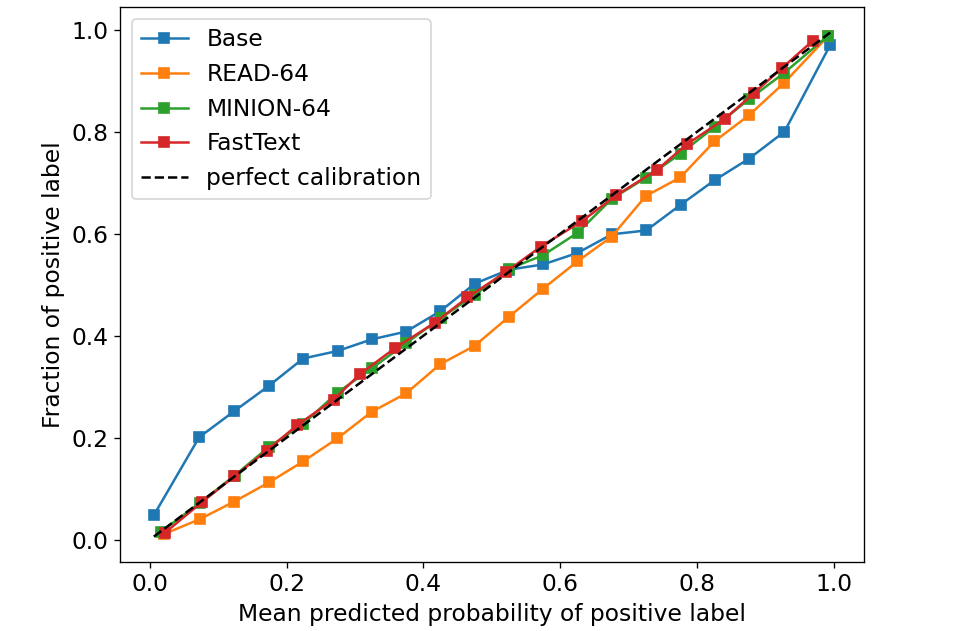
\includegraphics[width=\columnwidth]{calibration_plot_cropped.png}
    \caption{Calibration curves of the trained models for predicting positive sentiment. The dashed line represents the ideal model calibration. Regions, where the calibration curve of a model lies under the dashed line, represent overconfidence of the model in its predictions, and regions where it lies above represent underconfidence.}
    \label{fig:calibration-plots}
\end{figure}

\section{Discussion}
\label{sec:discussion}

% accuracy and energy consumption
BERTweet achieves the highest accuracy on the test set but is ahead of the other transformer-based models by less than one percent. MINION-8, 64, and 256 respectively only require about 52\%, 57\% and 71\% of the energy required for fully fine-tuning BERTweet. The low-cost alternative FastText achieves much lower accuracy but only requires negligible resources. \\
% compare read and minion accuracy
The MINION models also show slightly higher accuracy compared to READ for each hidden unit size respectively, while requiring less energy and memory utilisation during training. One should note that our implementations of READ and MINION are not optimized, and thus this marginal improvement of energy consumption and memory utilization is tentative and may also relate to the internal implementation of each model.\\
% calibration
The calibration errors in Table~\ref{tab:results} clearly show an improvement in the model calibration of all models compared to BERTweet on both ACE and MCE. This suggests that model calibration is significantly improved when using recurrent side models compared to full fine-tuning.
Comparing the calibration of READ to MINION, we can see a marked reduction in ACE and MCE. This could either be explained by the influence of the bidirectional GRU in each hidden layer of the transformer, or with the slight reduction in the number of parameters in MINION compared to READ. We can also observe a reduction in the ACE for MINION-8 compared to MINION-64. In line with previous findings \cite{guo2017calibration} this suggests, that larger models exhibit worse calibration. However, considering that here only two models are compared and only one dataset is evaluated, more research has to be done to find more definitive answers.

\section{Summary}
\label{sec:summary}
Overall, our implementation appears viable as a PETL method for sentiment classification, as it significantly reduces the computational cost required for training compared to full fine-tuning. MINION, by using a sequence-to-sequence RNN as a side model, further improves on READ \cite{read} achieving slightly higher accuracy with lower computational cost with the same number of hidden units. Finally, on this classification task, our approach shows much better calibration compared to full fine-tuning and slightly better calibration compared to READ. However, more research on different NLP tasks will be necessary, to confirm whether it performs well in general.

\bibliographystyle{IEEEtran}
\bibliography{report}
\end{document}
